\chapter{Crittografia a chiave pubblica} \label{ch:publickey}
\section{Introduzione}
La crittografia a chiave pubblica (\textbf{public key cryptography}), talvolta detta anche crittografia asimmetrica (\textbf{asymmetric cryptography}), fu pubblicamente introdotta nel 1975, anche se alcune voci sostengono che l'NSA già la utilizzasse da diverso tempo. Diversamente dalla crittografia a chiave segreta non prevede la \textbf{condivisione di un segreto}. Ogni entità ha due chiavi:

\begin{itemize}
	\item una chiave privata da \textbf{non rivelare} a nessuno
	\item una chiave pubblica da rivelare preferibilmente a tutto il mondo
\end{itemize}

\subsubsection{Terminologia e notazione}
Per convenzione si userà il termine \textbf{chiave privata} al posto di \textbf{chiave segreta}, per distinguere il concetto di chiave segreta utilizzata nel contesto di un algoritmo a crittografia simmetrica e chiave privata nel contesto di un algoritmo di crittografia asimmetrica. In base all'aggettivo della chiave sarà quindi immediato risalire allo schema di crittografia usato.
\begin{figure}[htbp]
	\centering%
	\subfigure%
	{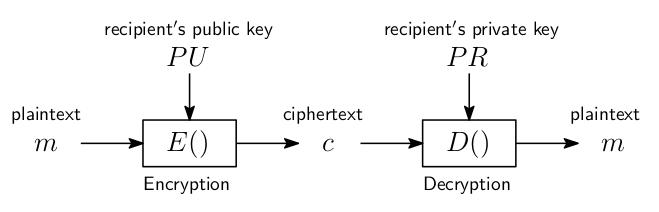
\includegraphics[height=13cm, width=10cm, keepaspectratio]{Immagini/chiave_pubblica/chiave_pubblica_schema.png}}
	\caption{Schema a blocchi crittografia a chiave pubblica \label{fig:pubblica_schema_blocchi}} 	
\end{figure}
Per quanto riguarda la notazione faremo riferimento alla \figurename~\ref{fig:pubblica_schema_blocchi}, in cui:
\begin{itemize}
	\item \textbf{PU} rappresenta la chiave \textbf{Pubblica}; ad esempio $PU_B$ indica la chiave pubblica di Bob
	\item \textbf{PR} rappresenta la chiave \textbf{Privata}; ad esempio $PR_B$ indica la chiave privata di Bob
\end{itemize}
Cifratura e decifratura sono due funzioni matematiche che sono l'una l'inverso dell'altra:
\begin{equation}
m = D(PR, c) = D(PR, E (PU, m))
\end{equation}

\subsubsection{Firma digitale}
La tecnologia a chiave pubblica consente anche di generare una \textbf{firma digitale} su un messaggio (ovvero garantirne l'autenticità). Basta infatti invertire il ruolo delle chiavi, come mostrato in \figurename~\ref{fig:pubblica_schema_firma}. In questo contesto le funzioni E() e D() vengono denominate S()(Sign) e V()(Verify). 
\begin{figure}[htbp]
	\centering%
	\subfigure%
	{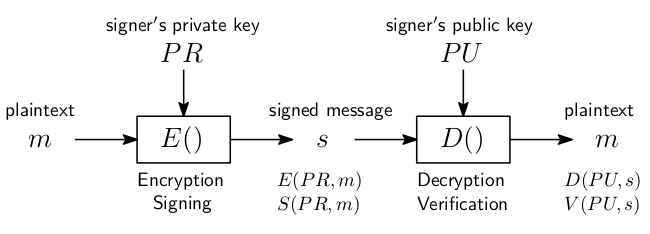
\includegraphics[height=13cm, width=10cm, keepaspectratio]{Immagini/chiave_pubblica/chiave_pubblica_firma.png}}
	\caption{Schema a blocchi crittografia a chiave pubblica \label{fig:pubblica_schema_firma}} 	
\end{figure}

La crittografia a chiave pubblica si basa su alcuni risultati nell'ambito della teoria dei numeri. Si esamineranno i seguenti schemi di cifratura a chiave pubblica: 
\begin{itemize}
\item RSA usata per cifrare e per calcolare la firma digitale
\item ElGamal e DSS, usati per la firma digitale
\item Diffie-Hellman, permette di stabilire un segreto condiviso, ma non fornisce alcun algoritmo che usa effettivamente tale segreto
\end{itemize}
L'unico aspetto comune a tutti gli algoritmi di crittografia a chiave pubblica è la presenza di due quantità correlate, una chiave segreta e una chiave pubblica, associate a ciascuna entità che partecipa ad una comunicazione cifrata. Spesso si usa il termine \textbf{principal} per fare riferimento a siffatta entità, che può essere un calcolatore o una persona.

\section{Aritmetica modulare}
La maggior parte degli algoritmi a chiave pubblica si basano sull'aritmetica modulare. Prima di affrontare tali algoritmi conviene quindi rivedere alcune definizioni.
\newline \newline
Supponiamo che $a$ e $b$ siano interi ($a,b \in \mathbb{Z}$), e $n$ sia un intero positivo ($n \in \mathbb{N}$). Allora 
\begin{defin}
Scriviamo: $a \equiv b(mod \; n)$, leggendo tale espressione \textit{"\textbf{a} è \textbf{congruente} a \textbf{b} modulo \textbf{n}"} se $n$ divide $b-a$
\end{defin}
Supponiamo di dividere \textit{a} e \textit{b} per \textit{n}, ottenendo quozienti interi e resti (con i resti tra \textit{0} e \textit{n - 1}). Avrò quindi:
\begin{equation}
a = q_a n + r_a
\end{equation}
\begin{equation}
b = q_b n + r_b
\end{equation}
Allora è facile mostrare che:
\begin{equation}
a \equiv b(mod \; n) \Leftrightarrow r_a = r_b
\end{equation}
Useremo quindi l'espressione $a$ mod $n$ per indicare il resto della divisione tra $a$ e $n$. Allora:
\begin{equation}
a \equiv b(mod \; n) \Leftrightarrow a(mod \; n) = b(mod \; n)
\end{equation}
Possiamo ora dare la seguente:
\begin{defin}
Un'aritmetica modulo n, denotata con $\mathbb{Z}_n$ è l'insieme {0,1,...,n-1}, dotato di due operazioni: l'addizione, denotata con il simbolo +, e la moltiplicazione, denotata con il simbolo x.
\end{defin}
In termini pratici, fissato un intero $ n>1 $, l'aritmetica modulare considera l'insieme degli interi non negativi minori di $n: $\{$0, 1, 2,..., n-1$\}, effettua operazioni ordinarie come l'addizione e la moltiplicazione, e sostituisce il risultato $x$ con il resto $r$ della divisione intera di $x$ per $n$. Il risultato finale viene detto modulo n o $mod \, n$. 

\paragraph{Addizione}
Consideriamo l'addizione mod 10. Siano a e b due numeri minori di 10. $(a + b)mod10$ si ottiene effettuando l'addizione ordinaria, e considerando come risultato finale la cifra meno significativa (cioè il resto della divisione per 10). L'addizione gode delle seguenti:
\begin{prop}[(Chiusura dell'addizione)]
$\forall a,b \in \mathbb{Z}$, $a + b \in \mathbb{Z}_n$ 
\end{prop}
\begin{prop}[(Commutativa)]
$\forall a,b \in \mathbb{Z}$, $a + b = b + a$ 
\end{prop}
\begin{prop}[(Associativa)]
$\forall a,b,c \in \mathbb{Z}$, $(a + b) + c = a + (b + c)$ 
\end{prop}
\begin{prop}[(Elemento neutro)]
$\forall a \in \mathbb{Z}$, $a + 0 = 0 + a = a$ 
\end{prop}
Sia m (< 10) un qualche messaggio. L'addizione di una costante k mod 10 può essere interpretata come una cifratura a chiave segreta, in cui:
\begin{itemize}
\item ogni cifra decimale \textbf{m} viene mappata in una diversa cifra decimale \textbf{c = (m + k) mod 10} in modo \textbf{reversibile}.
\item \textbf{k} è la \textbf{chiave segreta}; chiaramente si tratta di un pessimo cifrario (è il cifrario di Cesare)
\item la decifratura consiste nel sottrarre k mod 10, ovvero va sottratto k e se il risultato è minore di 0 va aggiunto 10
\item come nell'aritmetica ordinaria, sottrarre k equivale a sommare -k, cioè l'inverso additivo di k
\end{itemize}

\paragraph{Inverso additivo modulo n}
Un inverso additivo di k è un numero che sommato modulo n a k dà 0; formalmente: 
\begin{equation}
-k \mid -k \in \mathbb{N},\; -k < n,\; (k + (-k)) \, mod \, n = 0 \, mod \, n
\end{equation}
Ad esempio, l'inverso additivo di 4 è 6, perché 4 + 6 = 0 nell'aritmetica modulo 10.

\paragraph{Moltiplicazione modulare}
La moltiplicazione gode delle seguenti:
\begin{prop}[(Chiusura della moltiplicazione)]
$\forall a,b \in \mathbb{Z}$, $ab \in \mathbb{Z}_n$ 
\end{prop}
\begin{prop}[(Commutativa)]
$\forall a,b \in \mathbb{Z}$, $ab = ba$ 
\end{prop}
\begin{prop}[(Associativa)]
$\forall a,b,c \in \mathbb{Z}$, $(ab)c = a(bc)$ 
\end{prop}
\begin{prop}[(Elemento neutro)]
$\forall a \in \mathbb{Z}$, $a \times 1 = 1 \times a = a$ 
\end{prop}
\begin{prop}[(Distributiva)]
$\forall a,b,c \in \mathbb{Z}$, $(a + b)c = ac + bc$ 
\end{prop}
Anche in questo caso consideriamo anche in questo caso l'aritmetica modulo 10, facendo riferimento alla tabella \ref{fig:molt_mod}. Anche in questo caso l'operazione di moltiplicazione per una costante (come vedremo, per determinate costanti) può essere utilizzata per implementare una cifratura a chiave segreta.
\begin{figure}[htbp]
	\centering%
	\subfigure%
	{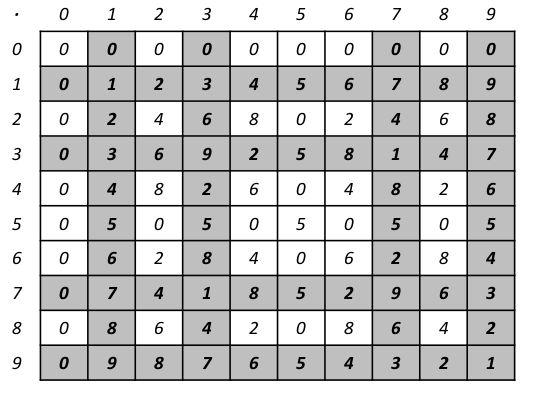
\includegraphics[height=7cm, width=7cm, keepaspectratio]{Immagini/chiave_pubblica/molt_mod.png}}
	\caption{Tabella moltiplicazione modulo 10 \label{fig:molt_mod}} 	
\end{figure}
Il problema, in questo caso, consiste nella possibilità di rendere invertibile l'operazione. Ad esempio, se si prova a cifrare moltiplicando per 5, metà dei numeri sarebbero cambiati in 0 e l'altra metà in 5. Ciò comporta una perdita di informazione $\Rightarrow$ la trasformazione non è invertibile $\Rightarrow$ è impossibile decifrare.
\newline \newline
In altre parole, poiché la decifratura può essere eseguita moltiplicando per l'inverso moltiplicativo di k, la possibilità di decifrare dipende dall'esistenza di tale inverso. Mentre l'inverso additivo di un numero k esiste sempre, stesso discorso non può essere fatto per l'inverso moltiplicativo. Approfondiamo questo concetto. 
\newline \newline
Si noti che nell'aritmetica ordinaria l'inverso moltiplicativo di $k$ è $\frac{1}{k}$, che in generale è una quantità frazionaria. Nell'aritmetica modulare si considerano solo numeri interi.

\paragraph{Inverso moltiplicativo modulo n}
Definiamo l'inverso moltiplicativo di $k$, indicato con $k^{-1}$, come quel numero che moltiplicato per $k$ dà 1, cioè:
\begin{equation}
k^{-1} \mid k^{-1} \in \mathbb{N}, \; k^{-1} < n,\; kk^{-1} \, mod \, n = 1 \, mod \, n
\end{equation}
Fissato $n$, non tutti i numeri hanno un inverso moltiplicativo $mod \, n$. Si prenda come esempio $n = 10$. Solo i numeri $\{1,3,7,9\}$ hanno un inverso moltiplicativo. Ad esempio:
\begin{equation}
7 \cdot 3 \, mod \,n = 1 \, mod \, n \Rightarrow 7^{-1} = 3
\end{equation}
Facendo riferimento all'utilizzo dell'operazione per l'implementazione di un algoritmo di cifratura, la cifratura potrebbe essere rappresentata dalla moltiplicazione per 7, e la decifratura dalla moltiplicazione per 3.
\newline \newline
Si osservi inoltre che, se $k$ ammette un inverso moltiplicativo $mod \, n $, esiste un unico inverso moltiplicativo $k^{-1} < n$. La moltiplicazione $mod \, n$ di per sé non costituisce un cifrario sicuro, ma funziona, nel senso che la moltiplicazione per $k$ produce un mescolamento dell'input.
\newline \newline
Trovare un inverso moltiplicativo $k^{-1}$ nella aritmetica $mod \, n$, \textbf{non è affatto banale} se $n$ è molto grande. Esiste un modo efficiente per risolvere tale problema, noto come \textbf{algoritmo di Euclide}, la cui efficacia è garantita dal seguente Teorema: 
\begin{thm}[di Euclide] \label{eq:euclide}
Dati $x$ ed $n$, con $x<n$, l'algoritmo di Euclide trova il numero $y<n$ tale che $xy \, mod \, n = 1$, ammesso che un siffatto $y$ esista.
\end{thm} 

Ha senso allora chiedersi quali sono dunque i numeri che hanno un inverso moltiplicativo $mod \, n$. Un numero x < n detiene un inverso moltiplicativo se e solo se x è relativamente primo con n. Formalmente:
\begin{equation}
x \mid x \in \mathbb{N},\; x < n,\; MCD(x,n) = 1
\end{equation}
Se $n$ è un numero primo, tutti gli interi da 1 a $n-1$ sono relativamente primi con $n$, quindi tali numeri ammettono tutti un inverso moltiplicativo $mod \, n$.

\subsection{Funzione di Eulero o totiente}  

Dato un intero \textbf{n} > 1, si definisce funzione $\varphi$ di Eulero, o \textbf{funzione totiente}, la funzione che associa ad \textbf{n} il numero $\varphi (n)$ degli interi positivi $i < n$ e relativamente
primi con n, cioè:
\begin{equation}
\varphi (n): \mathbb{N} \Rightarrow \mathbb{N} \mid \quad \varphi (n) = \mid \{ i \in \mathbb{N}, 0 < i < n: MCD(i,n) = 1 \} \mid
\end{equation}

Se $n$ è primo, tutti gli interi da 1 a $n-1$ sono relativamente primi con $n$. Ne segue che $\varphi(x) = n - 1$. Se $n = p \cdot q$, dove p e q sono numeri primi maggiori di 1, allora $\varphi(n) = (p-1)(q-1)$. Dimostriamo questa affermazione.

\paragraph{Dimostrazione} Adottiamo la seguente notazione:
\begin{itemize}
\item $N_{<n}$ :\{ 1, 2, ..., n-1\}
\item $M_p$: \{ $p \cdot 1$, $p \cdot 2$, ..., $p \cdot (q-1)$\} $\subset N_{<n}$ (multipli di p minori di n)
\item $M_q$: \{ $q \cdot 1$, $q \cdot 2$, ..., $(p-1) \cdot q$\} $\subset N_{<n}$ (multipli di q minori di n)
\end{itemize}
Allora posso esprimere il risultato della funzione totiente come la totalità dei numeri minori di n, tranne quelli che sono multipli di p o q:
\begin{equation}
\varphi (n) = \mid N_{<n} - M_p \cup M_q \mid
\end{equation}
Ne segue:
\begin{equation} \label{eq:tot1}
\varphi (n) = \mid N_{<n} \mid - \mid M_p \mid - \mid M_q \mid + \mid M_q \cap M_p \mid
\end{equation}
Poiché p e q sono numeri primi, il loro minimo comune multiplo sarà proprio $p \cdot q = n$, quindi:
\begin{equation}
M_q \cap M_p = \varnothing \Rightarrow \mid M_q \cap M_p \mid = 0
\end{equation}
Allora la \ref{eq:tot1} diventa:
\begin{equation}
\varphi (n) = \mid N_{<n} \mid - \mid M_p \mid - \mid M_q \mid 
\end{equation}
\begin{equation}
\varphi (n) = n-1 - (q -1) - (p - 1) =  p \cdot q - p - (q - 1) =  p \cdot (q - 1) - (q - 1)
\end{equation}
E diventa, come volevasi dimostrare:
\begin{equation}
\varphi (n) = (p - 1)(q - 1)
\end{equation}

\paragraph{Esponenziazione modulare}
L'esponenziazione modulare, o elevamento a potenza modulare, è simile a quella ordinaria: si esegue l'esponenziazione ordinaria e si considera il resto della divisione per n (ad esempio, $4^6 \; mod \; 10 = 6 \; mod \; 10$ poiché $4^6 = 4096$ e $4096 \; mod \; 10 = 6$
\newline \newline 
L'esponenziazione modulare gode della seguente:
\begin{prop} \label{prop:exp1}
$(x^a \, mod \, n)^b \, mod \, n \, =  (x^{a})^b \, mod \, n =  \, x^{ab} \, mod \, n$
\end{prop}
Analogamente a quanto visto per addizione e moltiplicazione modulare, quando l'esponenziazione è iniettiva, essa può essere utilizzata come algoritmo di cifratura. La decifratura può ottenersi ricorrendo al logaritmo discreto
(inverso dell'esponenziazione). Come nel caso della moltiplicazione, nell'esponenziazione modulare non tutti i numeri ammettono un logaritmo discreto.
\begin{figure}[htbp]
	\centering%
	\subfigure%
	{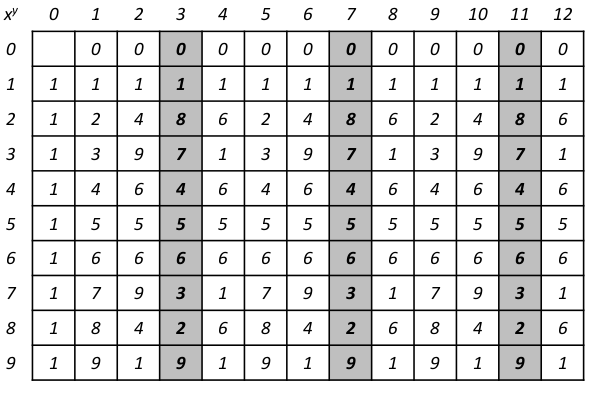
\includegraphics[height=7cm, width=7cm, keepaspectratio]{Immagini/chiave_pubblica/exp_mod.png}}
	\caption{Tabella esponenziazione modulo 10. E' facile vedere come l'esponenziazione per 3 (quarta colonna) possa considerarsi una cifratura, poiché determina un mescolamento dell'input. L'esponenziazione per 2, invece, no: alcuni input scompaiono (non è iniettiva) \label{fig:exp_mod}} 	
\end{figure}
\newline \newline
Esaminando la tabella di esponenziazione mod 10 in figura \ref{fig:exp_mod} si nota un periodicità: per ogni i > 0, le colonne i e i + 4 coincidono, cioè:
\begin{equation}
x^i \; mod \; 10 = x^{i + 4} \; mod \; 10, \quad \forall i>0
\end{equation}
In effetti, si può dimostrare il seguente risultato: sia $n > 1$ un intero privo di quadrati (cioè dove non compaiono fattori al quadrato nella sua scomposizione in fattori primi), detto anche \textbf{square free}, allora per ogni $y > 0$, si ha: 
\begin{equation}
x^y \, mod \, n = x^{(y + k\varphi(n) )} \, mod \, n
\end{equation} 
Dal precedente risultato segue che dato un numero $b = y + k\varphi(n)$ vale la seguente catena di uguaglianze:
\[
x^{b} \, mod \, n = x^{y} \, mod \, n = x^{b \, mod \, \varphi(n)} \, mod \, n
\]
Nel caso in cui $ b \, mod \, \varphi(n) = 1 \, mod \, \varphi(n) $, ovvero se $b = 1 + k \varphi(n) $, con $k \in \mathbb{Z}$, si ha:
\begin{equation}
x^b \, mod \, n = x \, mod \, n
\end{equation}
Tale risultato è sfruttato dall'algoritmo RSA.

\section{RSA}

RSA è un algoritmo di cifratura (a blocchi) a chiave pubblica, la cui lunghezza è variabile (solitamente si considerano chiavi di lunghezza pari ad almeno 512 bit). Anche la lunghezza dei blocchi è variabile: un blocco di testo in chiaro deve avere lunghezza minore di quella della chiave, mentre un blocco di testo cifrato è lungo come la chiave. \\
RSA è computazionalmente molto più lento degli algoritmi a chiave segreta più popolari come DES, IDEA e AES, per cui difficilmente viene usato per cifrare messaggi lunghi. Generalmente viene usato per cifrare una chiave segreta $K$, utilizzata per cifrare un messaggio usando un algoritmo a chiave segreta. RSA può essere usato dunque sia per cifrare/decifrare messaggi sia per la firma digitale di messaggi. In entrambi i casi bisogna disporre della coppia $<chiave \, pubblica, \,  chiave \, privata>(<PU,PR>)$. Nel seguito esamineremo:
\begin{enumerate}
\item generazione di una coppia $<PU,PR>$
\item cifratura/decifratura RSA
\item firma digitale RSA
\end{enumerate}

\subsection{Utilizzo di RSA} \label{sec:ut_rsa}

\paragraph{Generazione coppia di chiavi RSA}
I passi da seguire per generare la chiave pubblica e la chiave privata sono: 
\begin{enumerate}
\item Scegliere due numeri primi $p$ e $q$ molto grandi (circa 256 bit ciascuno) e porre $n = p \cdot q$. E' fondamentale che $p$ e $q$ rimangano segreti: fattorizzare $n$ è di fatto computazionalmente impraticabile. 
\item Scegliere un numero $e$ che sia relativamente primo rispetto a $\varphi(n) = (p-1)(q-1)$.
\item Calcolare l'inverso moltiplicativo $d$ di $e \, mod \, \varphi(n)$, cioè tale che sia $(d \cdot e ) \, mod \, \varphi(n) \, = 1$.
\item La chiave pubblica è $PU = <e,n>$, mentre la chiave privata è $PR = <d,n>$.
\end{enumerate}

\paragraph{Cifratura/Decifratura}
Per quanto riguarda la \textbf{cifratura}/\textbf{decifratura}, siano $PU = \langle e,n \rangle$ e $PR = \langle d,n \rangle$ la chiave pubblica e la chiave privata del destinatario e $m < n$ il messaggio da cifrare. La procedura da seguire è la seguente: 
\begin{itemize}
\item il mittente, utilizzando la chiave pubblica $PU$ del destinatario, cifra il messaggio ottenendo $c = m^e \, mod \, n$
\item il destinatario, usando la propria chiave privata $PR$, decifra $c$ calcolando $m = c^d \, mod \, n$. \end{itemize}

\paragraph{Dimostrazione dell'efficacia del procedimento}
Assunte come vere le seguenti proprietà: 
\begin{equation}\label{eq:eff_1}
m<n \Rightarrow \, m \, mod \, n\,=\,n
\end{equation}
\begin{equation} \label{eq:eff_2}
	x^{b} \, mod \, n = x^{b \, mod \, \varphi(n)} \, mod \, n
\end{equation}

E, poiché $d$ è l'inverso moltiplicativo di $e$:
\begin{equation} \label{eq:eff_3}
(e \cdot d) \, mod \, \varphi(n) = 1
\end{equation}
Allora, poiché:
\begin{equation}
c=E(PU,m) = m^e \, mod \, n
\end{equation}
Posso esprimere m in questo modo:
\begin{equation}
m=D(PR,c) = c^d \, mod \, n = (m^e \, mod \, n)^d \, mod \, n
\end{equation}
che, per la proprietà \ref{prop:exp1} dell'esponenziazione modulare (pag. \pageref{prop:exp1}), la \ref{eq:eff_3} e la \ref{eq:eff_3}, diventa:
\begin{equation}
m =  m^{ed} \, mod \, n = x^{ed \, mod \, \varphi(n)} \, mod \, n = m^{1 \, mod \, \phi(n)} \, mod \, n = m \, mod \, n
\end{equation}
e, infine, utilizzando la \ref{eq:eff_1} si ottiene, come volevasi dimostrare:
\begin{equation}
m = m \, mod \, n = m
\end{equation}

\paragraph{Firma digitale}
Per la \textbf{firma digitale} invece sia $PR$ la chiave privata del firmatario del messaggio e sia $PU$ la sua chiave pubblica: 
\begin{itemize}
\item il firmatario, usando la propria chiave privata $PR$, calcola la firma digitale $s = m^d \, mod \, n$;
\item chiunque desideri verificare l'autenticità della firma, può farlo usando la chiave pubblica $PU$ del firmatario e calcolando $m = s^e \, mod \, n$.
\end{itemize}
La dimostrazione dell'efficacia del procedimento è analoga a quella svolta per la cifratura/decifratura.

\subsection{Firma e cifratura di grandi messaggi} Abbiamo visto che affinché i processi i cifratura/decifratura e di firma/verifica siano efficaci è necessario che sia soddisfatta l'ipotesi:
\begin{equation}
|m| < n
\end{equation}
Dove |m| è la lunghezza del messaggio da processare. Per poter processare quindi messaggi di lunghezza qualsiasi non posso utilizzare solo RSA.

\paragraph{Firma di messaggi di lunghezza qualsiasi}
Per poter rispettare l'ipotesi sulla lunghezza del messaggio si può firmare, anziché l'intero messaggio, una sua impronta, come mostrato in figura \ref{fig:pubblica_schema_firma_grandi}
\begin{figure}[htbp]
	\centering%
	\subfigure%
	{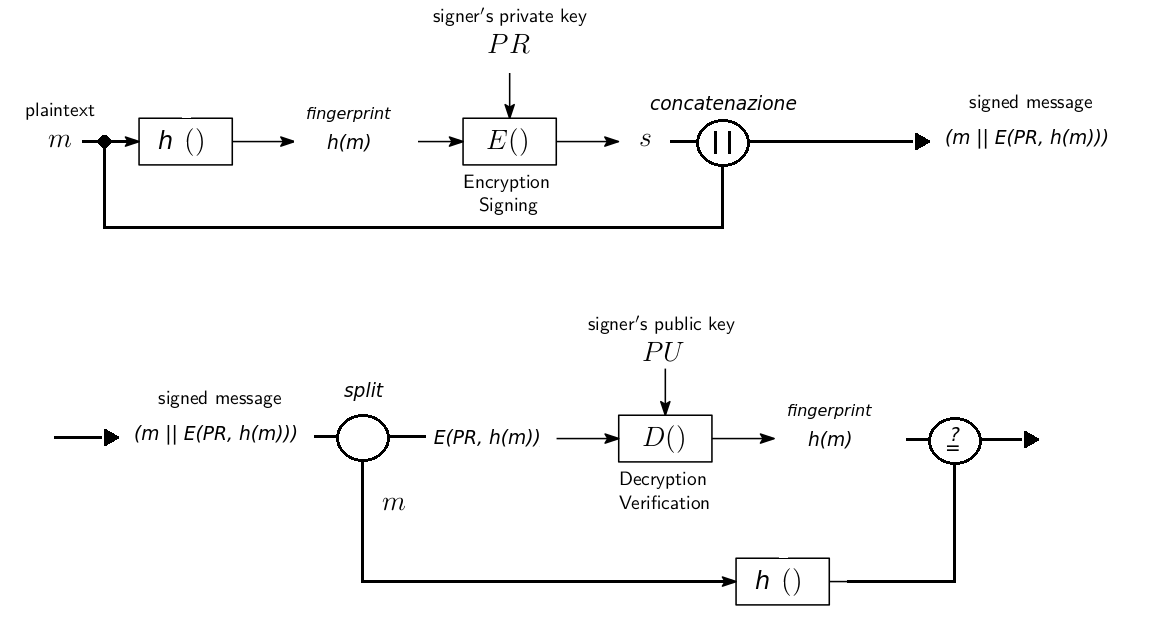
\includegraphics[height=15cm, width=15cm, keepaspectratio]{Immagini/chiave_pubblica/chiave_pubblica_firma_grandi.png}}
	\caption{Schema a blocchi crittografia a chiave pubblica - firma di grandi messaggi \label{fig:pubblica_schema_firma_grandi}} 	
\end{figure}

\paragraph{Cifratura di messaggi di lunghezza qualsiasi}
Per quanto riguarda la cifratura posso seguire la seguente procedura (figura \ref{fig:pubblica_schema_grandi}):
\begin{itemize}
\item cifrare il messaggio con una tecnologia a chiave segreta, in una delle modalità operative viste, utilizzando una chiave generata al momento
\item cifrare la chiave segreta generata con la chiave pubblica del destinatario
\item inviare la concatenazione delle due cifrature
\end{itemize}
\begin{figure}[htbp]
	\centering%
	\subfigure%
	{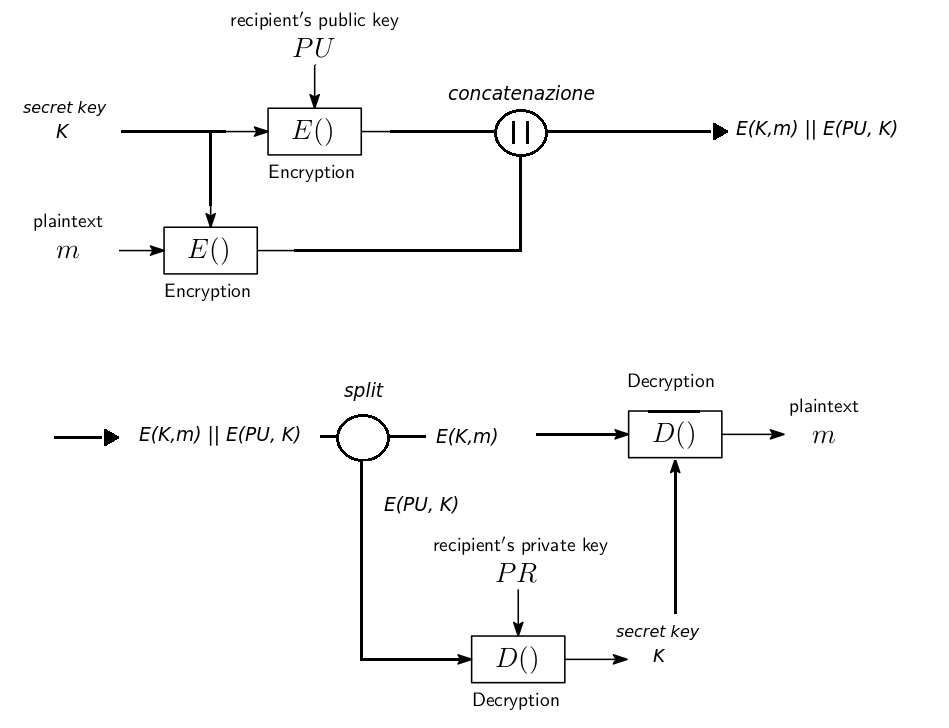
\includegraphics[height=15cm, width=15cm, keepaspectratio]{Immagini/chiave_pubblica/chiave_pubblica_schema_grandi.png}}
	\caption{Schema a blocchi crittografia a chiave pubblica - cifratura di grandi messaggi \label{fig:pubblica_schema_grandi}} 	
\end{figure}
\subsection{Sicurezza RSA}

La sicurezza di RSA deriva dal fatto che fattorizzare interi molto grandi è impraticabile. Infatti, se esistesse un metodo per identificare i numeri primi $p$ e $q$ tali che $n = p \cdot q$ (fattorizzazione di n), si otterrebbe $\varphi(n) = (p-1)(q-1)$ e quindi si potrebbe calcolare $d$ come l'inverso moltiplicativo di $e \, mod \, \varphi(n)$, ottenendo la chiave privata $PR = <d,n>$ dalla chiave pubblica $PU = <e,n>$. 
\newline \newline
Tuttavia è possibile violare RSA senza ricorrere alla fattorizzazione, se lo si usa in modo improprio. \\
In base al tipo di impiego, RSA svolge le seguenti operazioni\textbf{ molto frequentemente} (ad ogni sessione di lavoro): 
\begin{itemize}
\item cifratura/decifratura
\item generazione/verifica di una firma digitale
\end{itemize}
E' necessario pertanto che tali operazioni siano svolte nel modo \textbf{più efficiente possibile}. L'operazione di generazione delle chiavi viene invece eseguita meno frequentemente e quindi si può tollerare una minore efficienza.
\newline \newline
Le operazioni di cifratura, decifratura, firma e verifica della firma richiedono tutte di dover considerare un intero molto grande, elevarlo ad un esponente (intero) molto grande e trovare il resto della divisione intera per un numero molto grande. Considerando la dimensione dei numeri interi per i quali RSA è ritenuto sicuro, tali operazioni risulterebbero proibitive se eseguite nel modo più ovvio. Vanno quindi implementati algoritmi efficienti che svolgono tali operazioni.
\newline \newline
Va considerato però che problematiche di sicurezza possono insorgere anche da usi impropri dell'algoritmo. In altre parole vanno considerate le violazioni che non affrontano il problema della fattorizzazione. Si consideri, come esempio, un'applicazione di RSA con chiavi a 256 bit.
\newline \newline
Si supponga che Carol mandi un messaggio ad Alice contenente un il nome del suo amante. Il fidanzato di Carol, Bob, sapendo del messaggio di Carol ad Alice, e sapendo che l'amante di Carol è uno dei 15 studenti del corso di sicurezza informatica, potrebbe sferrare un attacco. Infatti, pur non potendo decifrare il messaggio, potrebbe cifrare il nome di ogni ragazzo del corso con la chiave pubblica di Alice ed effettuare un confronto.
\newline \newline
Com'è possibile prevenire quest'attacco? In seguito descriveremo degli standard per utilizzare RSA in modo appropriato (sezione: \ref{sec:pkcs}). Per il momento una possibile risposta alla precedente domanda è la seguente: Carol può concatenare il nome del suo fidanzato con un numero random molto grande, diciamo a 64 bit. A questo punto Bob, anziché 15 tentativi, deve fare $15 \cdot 2^{64}$ tentativi. L'attacco diventa computazionalmente impraticabile.

\subsection{Generazione delle chiavi RSA}
La generazione delle chiavi RSA, la cui procedura è descritta nel primo paragrafo della sezione \ref{sec:ut_rsa}, è un'operazione poco frequente: in gran parte delle applicazioni della tecnologia a chiave pubblica deve essere eseguita soltanto una volta e non è richiesta la stessa efficienza delle altre operazioni RSA; deve comunque essere garantita un'efficienza ragionevole. 
\newline \newline
Per generare una coppia di chiavi $<PU,PR>$ è necessario trovare:
\begin{enumerate}
\item due numeri primi $p$ e $q$ molto grandi
\item due interi $d$ ed $e$ con le proprietà precedentemente descritte
\end{enumerate}

\paragraph{Trovare due numeri primi grandi p e q}
Esistono infiniti numeri primi, che tendono a diradarsi all'aumentare di $n$: estraendo un numero a caso, si ha che:
\begin{equation}
Pr \{\text{n primo}\} \approx \frac{1}{{\text{ln} \, n}} \approx \frac{1}{N_{b}}
\end{equation}

dove $N_{b}$ è il numero di bit utilizzato per rappresentare $n$. La densità dei numeri primi è inversamente proporzionale alla loro lunghezza in bit (o in cifre decimali). Ad esempio, per un numero $n$ a cento cifre decimali (dimensione usata in RSA), c'è una possibilità su 230 che esso sia primo. Pertanto, i passi da seguire per generare $p$ e $q$ sono i seguenti: 
\begin{enumerate}
\item estrai un numero dispari molto grande
\item verifica se tale numero è primo, in caso negativo ritenta (in media, sono necessari 230 tentativi per ottenere un numero primo)
\end{enumerate}
Tale strategia va bene se si dispone di un \textbf{test di primalità efficiente}: come è possibile testare se un intero $n$ è primo? Un metodo banale consiste nel dividere $n$ per tutti gli interi $ \le n^{1/2}$ e verificare che non ci sono divisori $> 1$, ma ciò richiederebbe diverse vite dell'universo. Prima del 2002 non esisteva un test di primalità deterministico efficace in tempo polinomiale. Nel 2002 è stato pubblicato il test di primalità deterministico AKS.

\paragraph{Test di primalità probabilistico di RSA}
RSA utilizza tuttavia un test di primalità probabilistico: non si può affermare con certezza che l'esito del test sia corretto. Tuttavia, la probabilità di errore può essere resa arbitrariamente piccola aumentando il tempo di test. Il test si basa sul teorema di Fermat che fornisce una \textbf{condizione necessaria} affinché un intero $n$ sia primo: 
\begin{equation}
n \; \text{è primo} \Rightarrow \forall a \in \mathbb{Z}, a^{n-1} \, mod \, n  = 1 \, mod \, n
\end{equation}
Si noti con attenzione che non vale però il viceversa: esistono degli interi $a$ per i quali, l'uguaglianza è verificata anche se $n$ è non primo. In virtù di tale teorema, dato un intero $n$, un possibile test di primalità può consistere nei seguenti passi: 
\begin{enumerate}
\item scegliere un intero $a<n$;
\item calcolare $a^{n-1} \, mod \,n$;
\item \begin{enumerate} \item [a.] se il risultato è diverso da 1 $ \Rightarrow n$ è certamente non primo.
						\item [b.] se il risultato è pari a 1 $\Rightarrow $ $n$ potrebbe essere primo, anche se non è sicuro (è stato dimostrato che, se $n$ è un intero random di circa cento cifre decimali, la probabilità di un falso positivo è di circa $10^{-13}$).
	  \end{enumerate}
\end{enumerate}
Si osservi che un errore nel test di primalità può  rendere \textbf{impossibile} la decifratura RSA di un messaggio e \textbf{più facile} l'identificazione della chiave privata. 
\newline \newline
Se una probabilità di errore pari a $10^{-13}$ non è ritenuta sufficiente, si possono effettuare più test con diversi valori di $a$. Si ha che:
\begin{equation}
Pr \{\text{falso positivo dopo k test} \} = (10^{-13})^k
\end{equation}

\paragraph{Numeri di Carmichael}
La probabilità di errore può quindi essere resa arbitrariamente piccola aumentando il numero di test. Tuttavia esistono numeri particolari, per cui il test dà sempre un verdetto errato. Un numero $n$ è detto di Carmichael se \textbf{non è primo} e se per ogni $a \le n$ risulta $a^{n-1} = 1 \, mod \, n$. Va considerato che i numeri di Carmichael sono talmente rari che è estremamente improbabile estrarli a caso. Tuttavia, a fronte di un piccolo costo computazionale aggiuntivo, è possibile migliorare il test di primalità precedente introducendo altri controlli che permettono di rilevare con maggior probabilità se n è non primo. Un test molto efficace è il test di primalità di Miller e Rabin.

\paragraph{Calcolo di d ed e}

Gli interi $d$ ed $e$ sono definiti nel seguente modo: 
\begin{itemize}
\item $e$ è un qualunque numero relativamente primo rispetto all'intero $\varphi(n) = (p-1)(q-1)$;
\item $d$ è l'intero tale che $e \cdot \, mod \, \varphi(n) = 1 \Rightarrow$ noto $e$, $d$ si calcola con l'algoritmo di Euclide (pagina \pageref{eq:euclide}). 
\end{itemize}
Esistono due strategie per il calcolo di $e$:
\begin{enumerate}
\item una volta ottenuti $p$ e $q$, si sceglie randomicamente $e$ e si testa se esso è relativamente primo con $(p-1)(q-1)$; in caso negativo si ritenta con un altro valore di $e$.
\item Non selezionare prima $p$ e $q$, al contrario, si sceglie prima $e$, per poi scegliere $p$ e $q$ tali che la quantità $(p-1)(q-1)$ sia relativamente prima con $e$.
\end{enumerate}
La sicurezza di RSA non viene messa in crisi se $e$ è scelto sempre allo stesso modo: $d$ continua ad essere imprevedibile se $p$ e $q$ non sono noti. Se $e$ è un intero piccolo o facile da calcolare, le operazioni di cifratura e di verifica della firma diventano più efficienti, cioè le operazioni che richiedono l'uso della chiave pubblica $PU = <e,n>$ sono più veloci, mentre risulta invariata l'efficienza delle operazioni che richiedono la chiave privata $PR = <d,n>$. Chiaramente, diversamente da $e$, non si può assegnare a $d$ un valore piccolo, sebbene ciò renderebbe molto più veloci le operazioni che usano la chiave privata $PR$. Infatti, la sicurezza di RSA verrebbe meno: così si renderebbe l'informazione vulnerabile ad attacchi a forza bruta, poiché $d$ è l'esponente privato, a differenza di $e$ che è esponente pubblico. 

\paragraph{e = 3}
Di solito si usa $e=3$, poiché è comodo lavorare con esponenti piccoli, in modo che il calcolo di $m^e \, mod \, n$ non sia computazionalmente costoso (il calcolo di $ m^3 \, mod \, n$ richiede soltanto due moltiplicazioni) e la cifratura sia efficiente (così come la verifica della firma). Non si può scegliere $e=2$, in quanto non è relativamente primo con $(p-1)(q-1)$, che è un numero pari. 
\newline \newline
La scelta $e=3$ comporta alcune vulnerabilità: 
\begin{itemize}
\item se il messaggio $m$ da cifrare rappresenta un \textbf{intero piccolo}, in particolare se $m < n^{1/3} \Rightarrow  c = m^e \, mod \, n = m^3 \, mod \, n = m^3 \Rightarrow$ un avversario può decifrare $c$ senza conoscere la chiave privata semplicemente estraendo la radice
cubica ordinaria di $c \Rightarrow m = c^{1/3}$. Tale vulnerabilità può essere rimossa eseguendo un padding random del messaggio tale che $m^3 > n$. Ciò garantisce che $m^3$ viene sempre ridotto $ mod \, n $.
\item se uno \textbf{stesso messaggio} $m$ viene inviato cifrato a \textbf{tre o più destinatari} aventi un esponente pubblico $e=3$, il messaggio in chiaro $m$ può essere decifrato conoscendo soltanto i tre messaggi cifrati $c_{1}$, $c_{2}$ e $c_{3}$ e le tre chiavi pubbliche $<3,n_{1}>$, $<3,n_{2}>$ e $<3,n_{3}>$: si supponga infatti che un avversario intercetti tre cifrature dello stesso messaggio $m$, cioè $c_{1}$, $c_{2}$ e $c_{3}$. Conoscendo anche le tre chiavi pubbliche $<3,n_{1}>$, $<3,n_{2}>$ e $<3,n_{3}>$ e utilizzando il teorema cinese del resto, l'avversario può calcolare  $m^3 \, mod \, n_{1} \, n_{2} \, n_{3}$. Essendo $m<n_{i}$, per $i=1,2,3 \Rightarrow m^3<n_{1} \cdot n_{2} \cdot n_{3}$, da cui si ricava che $m^3 \, mod \, n_{1} \, n_{2} \, n_{3} = m^3 \Rightarrow$ l'avversario può risalire ad $m$ estraendo una radice cubica ordinaria. Anche questa vulnerabilità può essere rimossa mediante un padding random, così si evita che uno stesso messaggio cifrato venga inviato a piu destinatari. 
\end{itemize}
Si osservi che nelle applicazioni pratiche di RSA, il messaggio $m$ è generalmente una chiave di un algoritmo di cifratura a chiave segreta e in ogni caso $m$ è molto più piccolo di $n$, per cui è sempre possibile aggiungere dei bit di riempimento (padding) in modo tale che il messaggio risultante presenti delle caratteristiche desiderate. Se per ogni destinatario il padding scelto è random, la precedente vulnerabilità viene rimossa; la vulnerabilità può essere rimossa anche usando come padding gli identificatori univoci (ID) dei destinatari. 
\paragraph{e = 65537}
Un'altra scelta possibile è $e=65537$. Infatti esso è pari a $2^{16}+1$, che è un numero primo, e rimuove o riduce del tutto le vulnerabilità viste nel caso $e=3$. La prima vulnerabilità con $e=3$ si ha se $m^3<n$ e nel caso $e=65537$ non ci sono molti valori di $m$ tali che $m^{65537} < n$, a meno che $n$ non sia molto più lungo di 512 bit, quindi l'estrazione della 65537-esima radice ordinaria di $m$ non costituisce una vulnerabilità seria. La seconda vulnerabilità con $e=3$ si ha se uno stesso messaggio $m$ cifrato è inviato a 3 destinatari e nel caso $e=65537$, lo stesso tipo di vulnerabilità si ha quando $m$ viene inviato a 65537 destinatari: non si può dire certo che si tratti di un messaggio segreto! Infine, la scelta di fissare a priori $e=3$ ha richiesto di scegliere $n$ in modo tale che $\varphi(n)$ e 3 fossero relativamente primi. Nel caso $e=65537$ conviene generare $p$ e $q$ come se $e$ non fosse prefissato e rigettare ogni valore di $p$ o $q$ che è uguale a $1 \, mod \: 65537$. Tale evento si verifica con una probabilità molto piccola, cioè $2^{-16}$. 

\subsection{Vulnerabilità}
In generale, sono presenti anche altri tipi di vulnerabilità: nel caso della firma digitale risulta che, per ogni numero $x < n$, $x$ è la firma digitale del messaggio:
\newline
\begin{equation}
m_{x} = x^e \,  mod \, n
\end{equation}
\newline 
Infatti, 
\newline
\begin{equation}
m_{x}^d \, mod \, n = (x^e \, mod \, n)^d \, mod \, n = x^{ed} \, mod \, n
\end{equation}
\newline 
\begin{equation}
m_{x}^d \, mod \, n = x^{1 \, mod \, \varphi(n)} \, mod \, n
\end{equation}
\newline
\begin{equation}
m_{x}^d \, mod \, n = x \, mod \, n = x
\end{equation}
\newline 
Quindi è banale falsificare la firma di qualcuno se il messaggio $m$ da firmare non interessa. La difficoltà sta però nel falsificare la firma di uno specifico messaggio. 
\newline
Generalmente, ciò che viene firmato (messaggio + padding) ha una struttura sufficientemente vincolata: vengono inseriti dei bit di riempimento organizzati in pattern regolari; la probabilità che un numero random costituisca un messaggio (padding incluso) valido è trascurabile, cioè è estremamente improbabile che un numero random contenga i pattern regolari di bit. Tuttavia, visto che i numeri in RSA sono molto grandi un avversario ha a disposizione molti tentativi, dunque i pattern di riempimento vanno scelti in modo opportuno.

\paragraph{Smooth Numbers}
Un altro problema presente nella cifratura a chiave pubblica è quello dei \textit{smooth numbers}. Intuitivamente, uno smooth number è un numero scomponibile nel prodotto di molti numeri primi \textbf{ragionevolmente piccoli} (non conviene usare una definizione assoluta, poiché un numero è piccolo o grande in base alle capacità di calcolo dell'avversario). Ad esempio, il numero 6056820 è più \textbf{smooth} del numero 6567587, poiché 
\begin{equation}
6056820 = 2^2 \cdot 3^2 \cdot 5 \cdot 7 \cdot 11 \cdot 19 \cdot 23
\end{equation}
mentre
\begin{equation}
6567587 = 13 \cdot 557 \cdot 907
\end{equation}
Si tratta di una vulnerabilità prevalentemente teorica, nella pratica difficilmente realizzabile, poiché richiede un'enorme capacità di calcolo, la raccolta di un numero elevato di messaggi firmati e molta fortuna (per l'avversario). 
\newline \newline
\textbf{Idea base}: dalle firme $s_{1}$ e $s_{2}$ dei messaggi $m_{1}$ ed $m_{2}$, è possibile calcolare le firme dei messaggi:
\begin{itemize}
\item $m_{1} \cdot m_{2}$
\item $m_{1}/m_{2}$
\item $m_{1}^j$
\item $m_{2}^k$ 
\item $m_{1}^j \cdot m_{2}^k$
\end{itemize} 
Ad esempio, conoscendo la firma $s_{1} = [m_{1}] = m_{1}^d \, mod \, n $, è possibile ottenere la firma di $m_{1}^j$ senza conoscere $d$ (ovvero senza conoscere la chiave privata). Infatti:
\begin{equation}
[m_1^j] = (m_{1}^j)^d \, mod \, n = (m_{1}^d)^j \, mod \, n = (m_{1}^d \, mod \, n)^j \, mod \, n
\end{equation} 
La dimostrazione per $m_{2}^k$  è ovviamente analoga, mentre per $[m_{1} \cdot m_{2}]$, conoscendo $[m_{1}]$ e $[m_{2}]$ e utilizzando la proprietà associativa della moltiplicazione:
\begin{equation}
[m_{1} \cdot m_{2}] = (m_{1}^d \cdot m_{2}^d) \, mod \, n = m_{1}^d \, mod \, n \cdot m_{2}^d \, mod \, n
\end{equation}
La prova per la divisione è analoga, mentre l'ultima proprietà deriva della precedenti.
\newline \newline 
Se un avversario riesce a collezionare molti messaggi firmati, può ottenere la firma di ogni messaggio $m$ esprimibile come prodotto e/o divisione di messaggi della collezione. In particolare, se ottiene le firme di due messaggi $m_{1}$ e $m_{2}$ tali che il rapporto $m_{1}/m_{2}=p$, dove $p$ è un numero primo, l'attaccante può calcolare la firma di $p$. Inoltre, se è abbastanza fortunato da raccogliere molte coppie di questo tipo, egli può calcolare la firma di molti numeri primi, quindi può falsificare la firma di ogni messaggio dato dal prodotto di ogni sottoinsieme di tali numeri primi ciascuno elevato ad una qualunque potenza. Con abbastanza coppie, può falsificare la firma di ogni messaggio rappresentato da uno \textbf{smooth number}. 
\newline \newline
Generalmente, ciò che si firma con RSA è un digest di messaggio, a cui si aggiungono bit tramite padding:
\begin{equation}
m^{*} = pad(h(m))
\end{equation} 
Se i bit di riempimento sono degli zeri, anzichè essere random, è piu probabile che $m^*$ sia uno smooth number. Invece, è estremamente improbabile che un numero random $mod \, n$ sia smooth: 
\begin{itemize}
\item con un padding a sinistra di soli zeri, l'intero da firmare $m_{p} = h(m)$ rimane piccolo, per cui il padding non riduce la probabilità che $m_{p}$ sia smooth;
\item con un padding a destra di soli zeri, $m_{p} = h(m) \cdot 2^k $ è un intero molto più grande, ma è divisibile per una potenza di due, quindi, analogamente, il padding non riduce la probabilità che $m_{p}$ sia smooth;
\item con un padding a destra random, l'intero da firmare $m_{p}$ è estremamente improbabile che sia smooth. 
\end{itemize}
Tuttavia, si espone RSA alla minaccia nota come problema della radice cubica.

\paragraph{Problema della radice cubica}
Si assuma che si è optato per padding a destra random per ridurre la probabilità che le firme prodotte siano smooth. Si ha l'inconveniente che, se l'esponente pubblico è $e = 3$, allora un attaccante può \textbf{virtualmente falsificare la firma di un qualsiasi messaggio}. Proviamo quest'affermazione.
\newline \newline
Supponiamo che un attaccante, Carol, voglia falsificare la firma di un qualche messaggio $m$ avente digest $h_{m}$. Allora Carol applica un padding a destra di $h_{m}$ di soli 0, ottenendo quindi:
\begin{equation}
p_{m} = <h_{m} \mid 00..00>
\end{equation}
Poi calcola la radice cubica ordinaria e la arrotonda all'intero più vicino:
\begin{equation}
r = round(p_{m}^{1/3})
\end{equation} 
ottenendo la firma falsificata di $m$. Infatti:
\begin{equation}
r^e = r^3 = p_{m}
\end{equation} 
ossia $h_{m}$ con un padding a destra che è apparentemente casuale.

\subsection{PKCS} \label{sec:pkcs}
Ogni applicazione di RSA (cifratura, decifratura e firma) può essere soggetta a diversi tipi di attacchi, che possono essere sventati con opportune contromisure, basate sulla scelta di un'opportuna codifica/formato (quindi padding) del messaggio da cifrare/firmare. A tal fine è stato definito uno standard, \textbf{PKCS} (Public-Key Cryptography Standard), che stabilisce le codifiche per:
\begin{itemize}
\item chiave pubblica RSA
\item chiave privata RSA
\item firma RSA
\item cifratura RSA di messaggi corti (tipicamente chiavi segrete)
\item firma RSA di messaggi corti (tipicamente digest)
\end{itemize}
Esistono 15 standard PKCS per le diverse situazioni in cui la cifratura a chiave pubblica viene utilizzata. Noi esamineremo solo PKCS1. Esso è stato concepito per far fronte alle seguenti minacce:
\begin{itemize}
\item cifratura di messaggi prevedibili;
\item smooth number per le firme;
\item destinatari multipli di un messaggio quando $e=3$;
\item cifratura di messaggi di lunghezza inferiore ad un terzo della lunghezza di $n$ quando $e=3$;
\item firma di messaggi dove l'informazione è posta nei bit più significativi ed $e = 3$.
\end{itemize}
PKCS definisce, tra le altre cose, uno standard per la formattazione di un messaggio da cifrare (e da firmare) con RSA, anche se questo non è l'impiego tipico dell'algoritmo (come già detto, di solito vengono cifrate chiavi segrete e firmati digest). 

\section{Diffie-Hellman}

Diffie-Hellman è il primo sistema a chiave pubblica utilizzato. Meno generale di RSA, non serve né a cifrare/decifrare né a firmare messaggi, ma permette lo scambio di chiavi, in chiaro e su una rete pubblica insicura, tra due entità (che chiameremo Alice e Bob) e quindi di accordarsi su un segreto (chiave) condiviso, \textbf{senza rivelarlo}. \textbf{Intercettando tutti i messaggi scambiati non si è quindi in grado di risalire al segreto condiviso}. Tale segreto non viene generato da una delle due entità, ma è il risultato dello scambio dei messaggi. In particolare, dopo essersi scambiati complessivamente due messaggi (in chiaro), che tutto il mondo può conoscere, Alice e Bob conosceranno il segreto condiviso $K_{AB}$, il quale verrà poi usato per proteggere la confidenzialità con tecniche di cifratura convenzionali.
\newline \newline
Diffie-Hellman è realmente usato per stabilire una chiave segreta condivisa in alcune applicazioni, ad esempio nell'ambito della cifratura dei dati inviati in una LAN. Si osservi comunque che Diffie-Hellman non incorpora alcuna forma di autenticazione, senza la quale si rischia di condividere il segreto con un impostore.  

\subsection{Algoritmo} 
\paragraph{Precondizione}
Alice e Bob condividono due numeri $p$ e $g$, dove $p$ è un numero primo grande e $g$ radice primitiva di $p$. $p$ e $g$ sono noti in anticipo e possono essere resi di dominio pubblico in una repository accessibile sia da Alice che da Bob, oppure possono essere generati dall'iniziatore della comunicazione, diciamo Alice, e trasmessi a Bob nel messaggio che gli invierà;
\paragraph{Fase 0}
La fase 0 viene eseguita dall'iniziatore della comunicazione qualora i numeri $p$ e $g$ non siano pubblici: Alice genera (o estrae da un suo archivio) una coppia di numeri $p$ e $g$ tali da soddisfare le proprietà sopra elencate; $p$ e $g$ possono essere subito inviati a Bob oppure possono essere trasmessi nella Fase 3A.
\paragraph{Fasi 1 - 2 - 3}
\begin{enumerate}
\item [A.] Generazione del segreto privato $s_{A}$: Alice (iniziatore comunicazione) genera un numero random $s_{A}<p$ di 512 bit, che non verrà mai inviato a Bob (Fase 1, N.B. $s_A$ \textbf{non} è la chiave condivisa). Successivamente calcola $T_{A}=g^{s_{A}} \, mod \,p$ (Fase 2) e lo invia (su una rete insicura) a Bob (Fase 3).
\item [B.] Generazione del segreto privato $s_{B}$: Bob genera $s_{B}<p$ di 512 bit, che non verrà mai inviato ad Alice (Fase 1, N.B. $s_B$ \textbf{non} è la chiave condivisa). Successivamente calcola $T_{B}=g^{s_{B}} \, mod \, p$ (Fase 2) e lo invia in rete ad Alice (Fase 3).
\end{enumerate}
Si noti che $T_A$ e $T_B$ possono essere rivelati a tutto il mondo senza inficiare la sicurezza dell'algoritmo.
\paragraph{Fase 4}
\begin{enumerate}
\item [A.] Alice calcola $K_{AB}=T_{B}^{s_{A}} \, mod \,p$;
\item [B.] Bob calcola $K_{BA}=T_{B}^{s_{B}} \, mod \, p$;
\end{enumerate}
L'aritmetica modulare garantisce che $K_{AB}=K_{BA}$. Infatti si ha:
\begin{equation}
K_{AB} = T_{B}^{s_{A}} \, mod \,p = ({g^{s_{B}} \, mod \, p})^{s_{A}} \, mod \,p
\end{equation}
\begin{equation}
K_{AB} = g^{s_{B}s_{A}} \, mod \, p = g^{s_{A}s_{B}} \, mod \, p
\end{equation} 
\begin{equation}
K_{AB} = ({g^{s_{A}} \, mod \, p})^{s_{B}} \, mod \,p = T_{A}^{s_{B}} \, mod \, p = K_{BA}
\end{equation}
\begin{figure}[htbp]
	\centering%
	\subfigure%
	{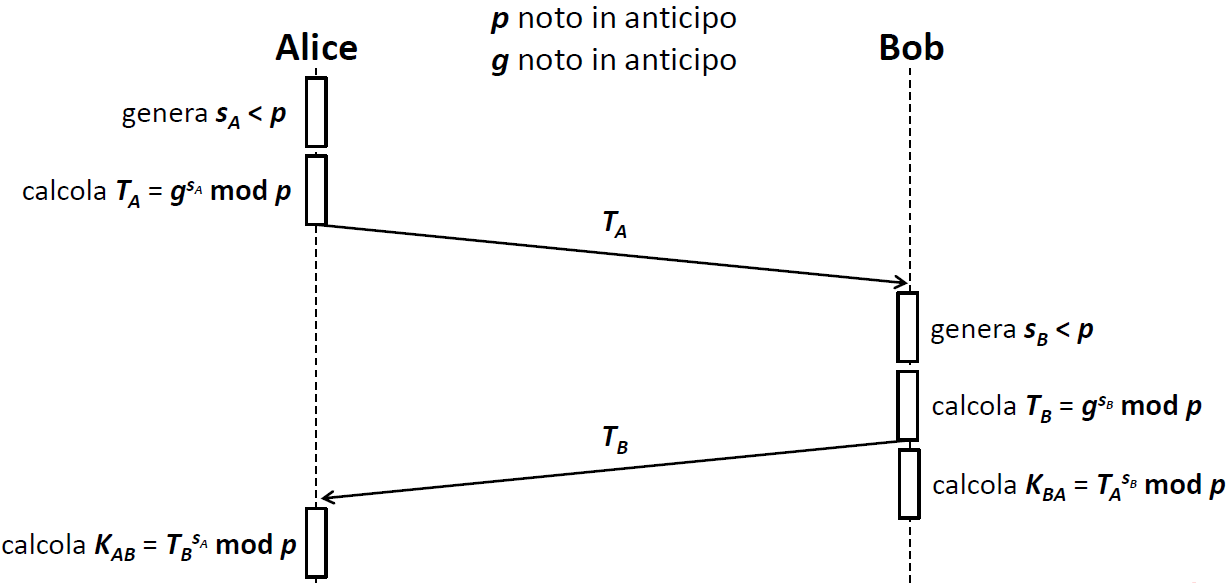
\includegraphics[scale=0.5, keepaspectratio]{Immagini/chiave_pubblica/DiffieHellman_schema.png}}
	\caption{Diffie-Hellman: schema}
\end{figure}

\paragraph{Sicurezza}
L'algoritmo non sarebbe sicuro se, dati $p$, $g$, $T_{A}$ e $T_{B}$ (trasmessi in chiaro), fosse possibile calcolare $s_{A}$, $s_{B}$ oppure $g^{s_{A}s_{B}}$. Al momento non sono note tecniche per calcolare $g^{s_{A}s_{B}}$ in tempo ragionevole, anche conoscendo $g^{s_{A}}$ e $g^{s_{B}}$. Di fatto si può ottenere $s_{A}$ da $g^{s_{A}}$ tramite logaritmo discreto:
\begin{equation}
dlog_{g} \, g^{s_{A}}, \quad dlog_{g}: \mathbb{Z} \rightarrow \mathbb{N}
\end{equation} 
Tuttavia il calcolo di logaritmi discreti non è fattibile in tempi ragionevoli.
\subsection{Man in the middle}
La vulnerabilità di Diffie-Hellman è che tale algoritmo non fornisce alcuna prova di autenticazione: Alice non può essere certa che $T_{B}$ sia stato inviato da Bob e non da un impostore; allo stesso modo, Bob non può essere certo che $T_{A}$ sia stato inviato da Alice e non da un impostore. 

\paragraph{Man in the middle} 
E' quindi possibile che un impostore, Mr. X, intercetti e modifichi i messaggi facendo credere a Bob di comunicare con Alice e viceversa. Alice e Bob non hanno modo di rendersi conto dell'attacco in atto. 
\newline \newline
Un attacco di questo tipo viene detto Man-in-the-Middle (o \textbf{Bucket Brigade Attack}): Alice pensa che $K_{AX}$ sia la chiave segreta $K_{AB}$ che condivide con Bob; Bob pensa che $K_{BX}$ sia la chiave segreta $K_{BA}$ che condivide con Alice; invece, Mr. X ha due chiavi segrete: 
\begin{itemize}
\item $K_{XA}$ per comunicare con Alice;
\item $K_{XB}$ per comunicare con Bob.
\end{itemize}
Questo perché Mr. X conosce $g$ e $p$, quindi si calcola $s_{x}<p$ e $T_{x}=g^{s_{x}} \, mod \, p$ e li invia sia ad Alice che a Bob. Tale attacco è un attacco all'integrità, alla confidenzialità e all'autenticità.
\begin{figure}[htbp]
	\centering%
	\subfigure%
	{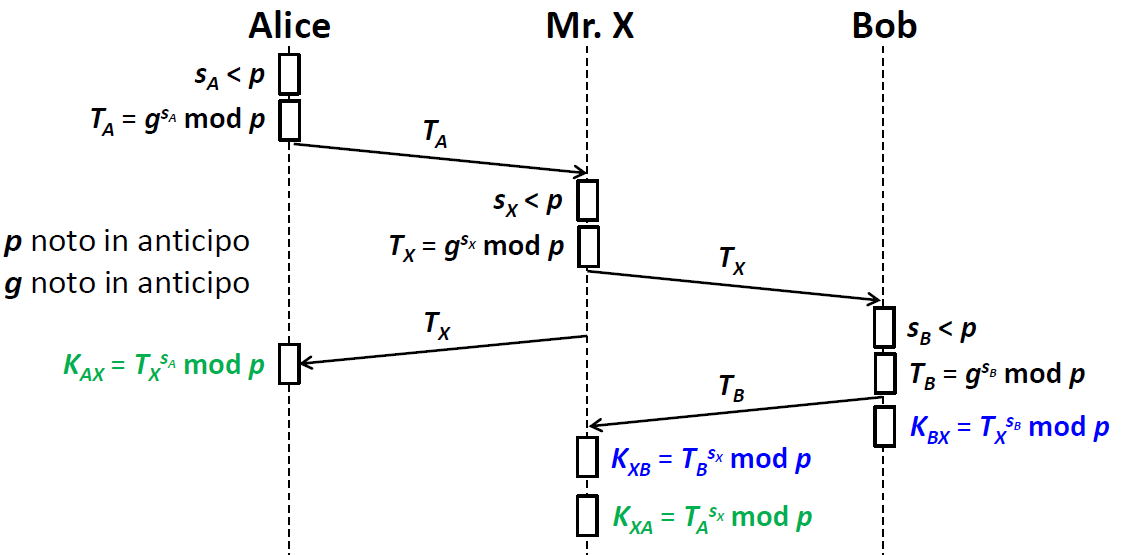
\includegraphics[scale=0.5, keepaspectratio]{Immagini/chiave_pubblica/DiffieHellman_maninthemiddle.png}}
	\caption{Man-in-the-Middle Attack}
\end{figure}

\subsection{Possibili soluzioni}
\paragraph{Autenticazione via password}
Assumiamo che Alice e Bob si siano preliminarmente accordati su una coppia di password ($pwd_{A}$, password che Alice invia a Bob, e $pwd_{B}$, password che Bob invia ad Alice). Si consideri allora la seguente procedura di autenticazione mostrata in \figurename~\ref{fig:aut_via_pwd}, dove $K_{AB}$ è la chiave segreta condivisa ottenuta con Diffie-Hellman: 
\begin{enumerate}
\item scambio chiavi Diffie-Hellman;
\item Alice invia un messaggio cifrato con $K_{AB}$ e $pwd_{A}$;
\item Bob invia un messaggio cifrato con $K_{BA}$ e $pwd_{B}$.
\end{enumerate}
\begin{figure}[htbp]
	\centering%
	\subfigure%
	{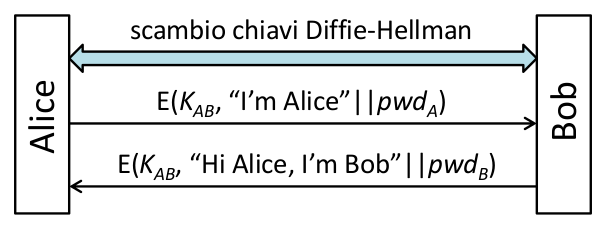
\includegraphics[scale=0.5, keepaspectratio]{Immagini/chiave_pubblica/DiffieHellman_auth0.png}}
	\caption{Autenticazione via password}
	\label{fig:aut_via_pwd}
\end{figure}
Il problema è che l'autenticazione via password, se è in corso un attacco Man-in-the-Middle, non funziona: Mr. X può decifrare tutte i messaggi che riceve da Alice con $K_{AX}$, cifrarli con $K_{XB}$ e inviarli a Bob. Viceversa, può decifrare tutte i messaggi che riceve da Bob con $K_{XB}$, cifrarli con $K_{AX}$ e inviarli ad Alice. In questo modo può anche venire a conoscenza delle password su cui Alice e Bob si erano preliminarmente accordati.
\begin{figure}[htbp]
	\centering%
	\subfigure%
	{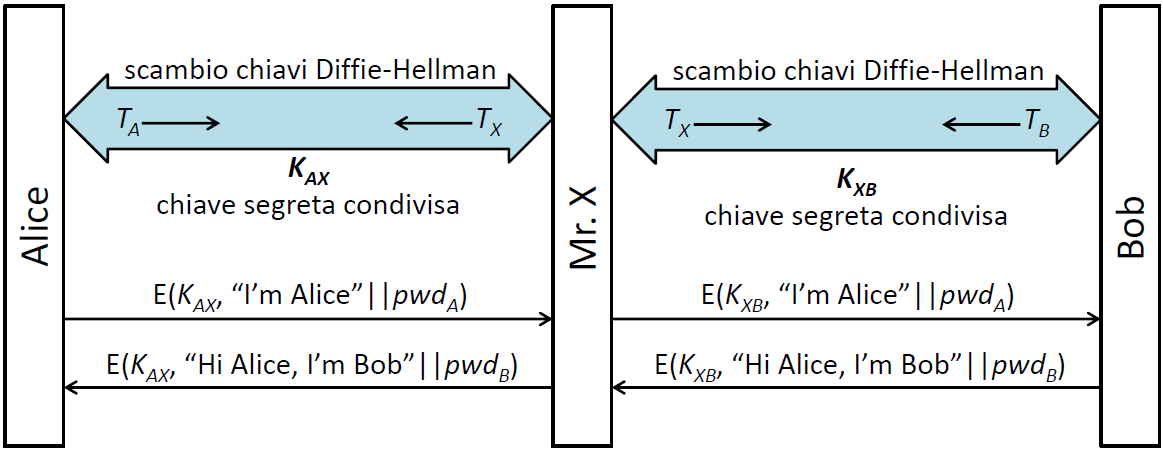
\includegraphics[scale=0.5, keepaspectratio]{Immagini/chiave_pubblica/DiffieHellman_passauth.png}}
	\caption{Autenticazione via password - Vulnerabilità}
	\label{fig:aut_via_pwd}
\end{figure}
Anche altri tipi di proposte sono insufficienti (timestamp, domande personali, ecc.). Il problema è che Diffie-Hellman effettua delle operazioni invertibili (cifratura/decifratura) ed è sicuro solo nel caso di attacchi passivi (un intruso intercetta i messaggi, ma non li modifica). E' necessario proteggere l'integrità, per cui si adottano due strategie generali: Diffie-Hellman con Numeri Pubblici e Scambio Diffie-Hellman Autenticato.	


\paragraph{Diffie-Hellman con Numeri Pubblici} Un possibile modo per sventare attacchi attivi è evitare che $p$, $g$, $s_{A}$, $s_{B}$, $T_{A}$ e $T_{B}$ vengano generati/calcolati ad ogni scambio. $p$, $g$, $T_{A}$ e $T_{B}$ potrebbero essere resi pubblici in una repository fidata, con $p$ e $g$ uguali per tutti gli utenti, mentre ogni utente U pubblica il proprio valore $T_{U}$, mantenendo privato il segreto $s_{U}$. Ne consegue che, se un avversario non è in grado di accedere alla repository e di modificare i valori pubblici, allora Diffie-Hellman diventa sicuro anche nel caso di attacchi attivi. Inoltre, non è più necessario lo scambio dei valori $T_{A}$ e $T_{B}$: consultando la repository ogni utente A può ottenere la chiave $K_{AB}$ che condividerebbe con l'utente B. 

\paragraph{Scambio Diffie-Hellman Autenticato}
La precondizione per l'attuazione di questo protocollo è la conoscenza, da parte di Alice e Bob, di un qualche tipo di informazione che permette loro di autenticarsi reciprocamente, ovvero una chiave segreta condivisa $K^{AB}$, da non confondere con la chiave concordata con Diffie-Hellman $K_{AB}$, la propria coppia <chiave privata, chiave pubblica> e la chiave
pubblica dell'altro. Si possono usare tale(i) informazione(i) per provare che sono realmente loro, e non un impostore, coloro che generano i valori di Diffie-Hellman $g$, $p$, $T_{A}$ e $T_{B}$. Tale prova può avvenire sia contestualmente che dopo lo scambio Diffie-Hellman esaminato in precedenza. 
\newline \newline
Notazione adottata: \begin{itemize}
\item $K^{AB}$: chiave segreta condivisa tra Alice e Bob prima di effettuare lo scambio Diffie-Hellman.
\item $K_{AB}$: chiave concordata con Diffie-Hellman.
\item $K^{AB}$ \{msg\} : cifratura di msg con la chiave segreta $K^{AB}$, cioè $E(K^{AB}, msg)$.
\item $\{msg\}_{Bob}$ : cifratura di msg con la chiave pubblica di Bob, cioè $E(PU_{Bob}, msg)$.
\item $[msg]_{Bob}$ : firma di msg con la chiave privata di Bob, cioè $E(PR_{Bob}, msg)$.
\end{itemize}
Di seguito sono indicate alcune possibili soluzioni per lo scambio Diffie-Hellman autenticato:
\begin{itemize}
\item Autenticazione \textbf{contestuale} allo scambio Diffie-Hellman: \begin{enumerate}
\item Cifrare lo scambio Diffie-Hellman con la chiave segreta $K^{AB}$ (\figurename~\ref{fig:auth1}).
\begin{figure}[htbp]
	\centering%
	\subfigure%
	{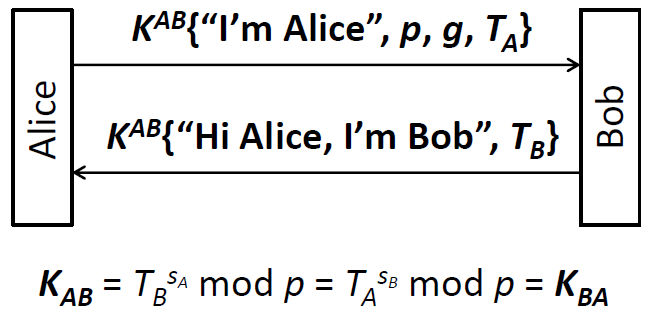
\includegraphics[scale=0.5, keepaspectratio]{Immagini/chiave_pubblica/DiffieHellman_auth1.png}}
	\caption{Utilizzo $K^{AB}$.}
	\label{fig:auth1}
	\end{figure}
\item Cifrare il valore Diffie-Hellman con la chiave pubblica dell'altro interlocutore (\figurename~\ref{fig:auth2}).
\begin{figure}[htbp]
	\centering%
	\subfigure%
	{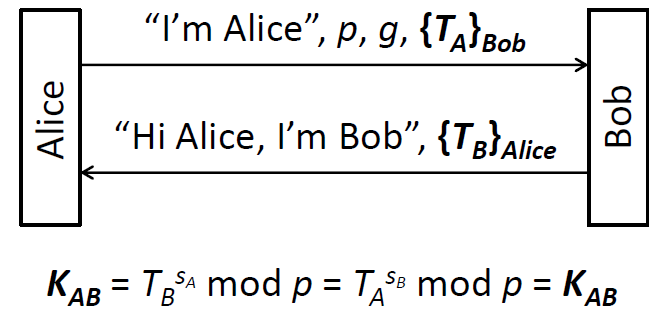
\includegraphics[scale=0.5, keepaspectratio]{Immagini/chiave_pubblica/DiffieHellman_auth2.png}}
	\caption{Utilizzo chiave pubblica dell'altro interlocutore.}
	\label{fig:auth2}
	\end{figure}
\item Firmare il valore Diffie-Hellman con la propria chiave privata (\figurename~\ref{fig:auth3}).
\begin{figure}[htbp]
	\centering
	\subfigure
	{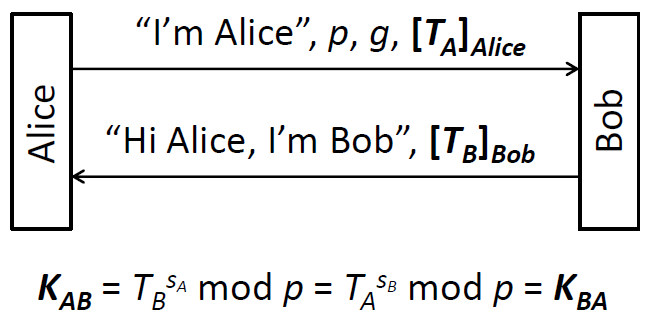
\includegraphics[scale=0.5, keepaspectratio]{Immagini/chiave_pubblica/DiffieHellman_auth3.png}}
	\caption{Utilizzo propria chiave privata.}
	\label{fig:auth3}
	\end{figure}
\end{enumerate}
\item Autenticazione \textbf{successiva} allo scambio Diffie-Hellman (\figurename~\ref{fig:auth45}):
\begin{enumerate}
\item Dopo lo scambio Diffie-Hellman, trasmettere un hash della chiave concordata $K_{AB}$, del proprio nome e della chiave segreta $K^{AB}$.
\item Dopo lo scambio Diffie-Hellman, trasmettere un hash del valore
Diffie-Hellman trasmesso e della chiave segreta $K^{AB}$.
\end{enumerate}
\end{itemize}
\begin{figure}[htbp]
	\centering
	\subfigure
	{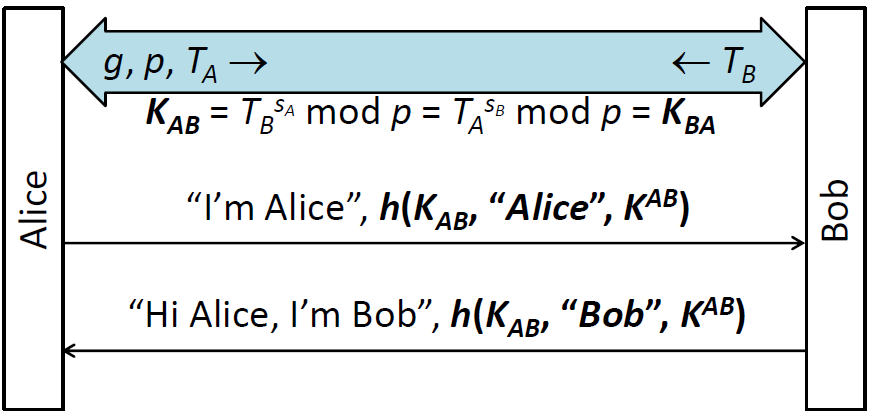
\includegraphics[scale=0.5, keepaspectratio]{Immagini/chiave_pubblica/DiffieHellman_auth4.png}}
	\hspace{2mm}
	\subfigure
	{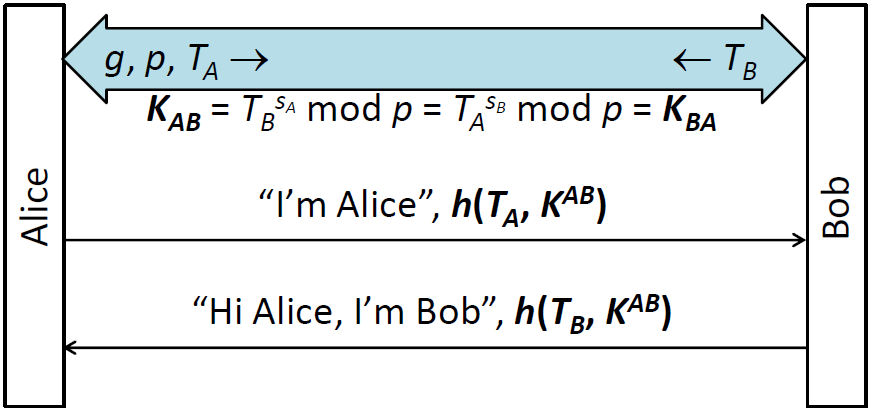
\includegraphics[scale=0.5, keepaspectratio]{Immagini/chiave_pubblica/DiffieHellman_auth5.png}}
	\caption{Autenticazione successiva allo scambio Diffie-Hellman.}
	\label{fig:auth45}
\end{figure}

Oltre alla mancanza di autenticazione, Diffie-Hellman classico presenta anche lo svantaggio che la comunicazione cifrata con la chiave concordata può avvenire soltanto dopo l'esecuzione di uno scambio attivo. In pratica, Alice non può inviare un messaggio cifrato a Bob prima di ricevere $T_{B}$. Tale problema puo essere ovviato introducendo le chiavi pubbliche Diffie-Hellman: una chiave pubblica D-H è una tripla $<p, g, T>$, dove $T = g^s \, mod \, p$, dove $s$ è la corrispondente chiave privata. Le chiavi pubbliche vanno custodite in un luogo fidato e accessibile da tutti in modo sicuro. La chiave pubblica di Bob è $<p_{B}, g_{B}, T_{B}>$. \newline \newline
Di seguito (\figurename~\ref{fig:authex}), mostriamo un esempio di procedura che consente ad Alice di inviare un messaggio cifrato a Bob, con la chiave concordata $K_{AB}$, anche se Bob risulta essere inattivo, cioè Alice deve essere in grado di cifrare senza dover attendere alcuna risposta da Bob. Bob, una volta attivo, dovrà poter calcolare $K_{AB}$ e decifrare il messaggio.
\begin{enumerate}
\item Alice genera $s_{A}<p_{B}$, calcola $T_{A}^{*}=g_{B}^{s_{A}} \, mod \, p_{B}$ e $K_{AB}=T_{B}^{s_{A}} \, mod \, p_{B}$.
\item Poi cifra il messaggio $msg=E(K_{AB},msg)$ e lo invia a Bob assieme a $T_{A}^{*}$.
\item Bob, una volta attivo, calcola  $K_{BA}=(T_{A}^*)^{s_{B}} \, mod \, p_{B}$.
\item Decifra $E(K_{AB},msg)$, ottenendo $msg=D(K_{BA},E(K_{AB},msg))$.
\end{enumerate}
\begin{figure}[htbp]
	\centering%
	\subfigure%
	{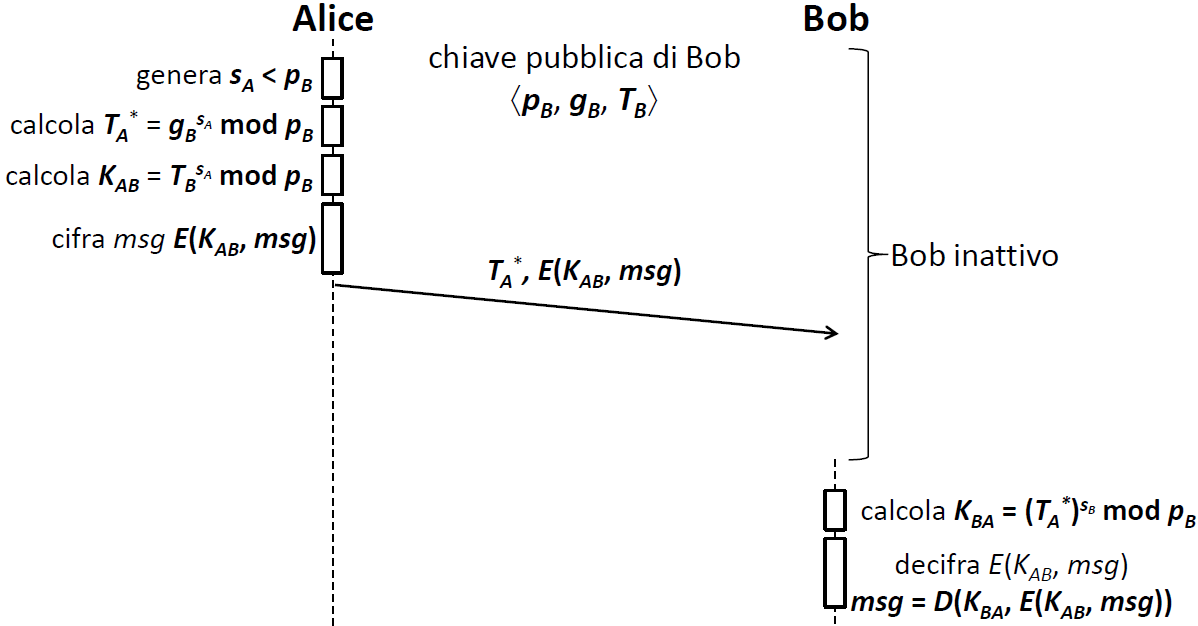
\includegraphics[scale=0.6, keepaspectratio]{Immagini/chiave_pubblica/DiffieHellman_pubseckey.png}}
	\caption{Chiavi pubbliche/private Diffie-Hellman}
	\label{fig:authex}
\end{figure} 

\section{Zero Knowledge Proof System}
La dimostrazione della conoscenza di un segreto è alla base di molte tecniche di autenticazione. Nelle tecniche di autenticazione a chiave segreta, il segreto è appunto la chiave condivisa tra i due principal. Nei protocolli a chiave pubblica il segreto è la chiave privata (associata alla chiave pubblica) nota solo ad un principal. \\
Una dimostrazione quindi è a \textit{conoscenza zero} (\textbf{Zero Knowledge Proof, ZKP}) se permette di provare la conoscenza di un segreto senza fornire delle informazioni che permettano ad un impostore di eseguire la prova: 
\begin{itemize}
\item la prova non deve rivelare il segreto;
\item la prova non deve rivelare eventuali informazioni, che pur non essendo il segreto, consentano comunque ad un impostore di effettuare la prova.
\end{itemize}
Le dimostrazioni a conoscenza zero sono impiegate nei protocolli/sistemi di autenticazione (detti \textbf{Zero Knowledge Proof Systems, ZKPS}). RSA è un esempio di ZKPS: è possibile provare la conoscenza di un segreto associato alla chiave pubblica (si pensi alla firma di una sfida), senza rivelare la chiave privata o altre informazioni che permettano ad un impostore di impersonare il proprietario della chiave privata. Tuttavia, esistono ZKPS molto più efficienti di RSA, anche se non permettono di cifrare e/o di firmare. 

\paragraph{La storia di Peggy e Victor}
In una dimostrazione a conoscenza zero sono sempre coinvolte due parti:
\begin{itemize}
\item il dimostratore \textbf{Peggy}: l'entità che dimostra di possedere il segreto
\item il verificatore \textbf{Victor}: l'entità che verifica la correttezza della prova
\end{itemize}
Peggy conosce la parola segreta per aprire la porta magica di una caverna, che si richiude automaticamente. La caverna ha la forma di un cerchio, con l'entrata su un lato e la porta magica che blocca l'altro lato (\ref{fig:peggy_victor_1}). Victor dice che la pagherà per il segreto, ma non fino a quando sarà sicuro che lei lo conosca veramente. Peggy dice che gli dirà il segreto, ma non prima di ricevere i soldi. Peggy deve dare quindi una dimostrazione a conoscenza zero. Pianificano quindi uno schema con il quale Peggy può provare di conoscere la parola senza dichiararla a Victor.
\begin{figure}[htbp]
	\centering%
	\subfigure%
	{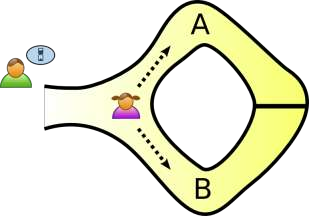
\includegraphics[height=5cm, width=5cm, keepaspectratio]{Immagini/chiave_pubblica/peggy_victor_1.png}}
	\caption{Storia di peggy e Victor\label{fig:peggy_victor_1}}
\end{figure}
Prima, Victor aspetta fuori dalla caverna mentre Peggy entra. Etichettiamo il sentiero sinistro e quello destro partendo dall'entrata con A e B. Peggy sceglie a caso uno dei due sentieri. Quindi, Victor entra nella caverna e grida il nome del sentiero che Peggy dovrà utilizzare per ritornare indietro, preso a caso. Se si ipotizza che lei conosca veramente
la parola magica, è facile: apre la porta, se necessario, e ritorna attraverso il sentiero desiderato. È da notare che Victor non conosce il sentiero per il quale Peggy è entrata.
\begin{figure}[htbp]
	\centering%
	\subfigure%
	{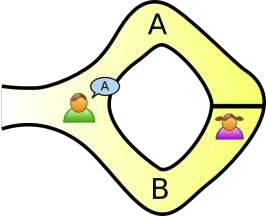
\includegraphics[height=5cm, width=5cm, keepaspectratio]{Immagini/chiave_pubblica/peggy_victor_2.png}}
	\caption{Storia di peggy e Victor\label{fig:peggy_victor_2}}
\end{figure}
\begin{figure}[htbp]
	\centering%
	\subfigure%
	{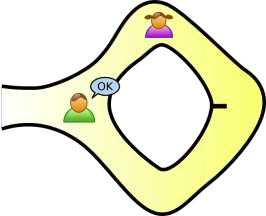
\includegraphics[height=5cm, width=5cm, keepaspectratio]{Immagini/chiave_pubblica/peggy_victor_3.png}}
	\caption{Storia di peggy e Victor\label{fig:peggy_victor_3}}
\end{figure}
Supponiamo che Peggy non conosca la parola. In questo scenario sarebbe in grado di tornare attraverso il sentiero chiamato se Victor avesse scelto il nome dello stesso sentiero per cui lei era entrata. Poiché Victor ha scelto A o B a caso, avrebbe il 50\% di probabilità di indovinare correttamente. Se i due ripetessero questo trucco molte volte, diciamo venti volte, una dopo l'altra, l'opportunità per Peggy di anticipare correttamente tutte le richieste di Victor diventerebbe statisticamente molto piccola (in virtù della probabilità di eventi indipendenti). Perciò, se Peggy appare in modo “affidabile” all'uscita
chiamata da Victor, questo può concludere che molto probabilmente conosca davvero la parola segreta.
\newline \newline
Uno schema di autenticazione a conoscenza zero (\textbf{Zero Knowledge Authenication Scheme, ZKAS}) consiste in un'autenticazione che sfrutta una \textbf{ZKP}. Non si tratta di una tecnica deterministica, ma \textbf{probabilistica} (anche RSA in fondo è probabilistica). Devono poter essere rese arbitrariamente piccole le probabilità che:
\begin{itemize}
\item un dimostratore onesto fornisca una prova errata
\item un verificatore onesto fornisca una verifica errata quando il dimostratore è onesto
\item un dimostratore disonesto fornisca una prova corretta
\end{itemize} 
Uno schema di autenticazione a conoscenza zero deve soddisfare i seguenti \textbf{requisiti}: 
\begin{itemize}
\item[a.] ad ogni entità è associato un segreto privato $s$ e
una chiave pubblica $k_{s}$, cioè una coppia $<s, k_{s}>$. Ovviamente, $k_{s}$ non deve esporre $s$;
\item[b.] l'autenticazione consiste nel provare la conoscenza del segreto $s$;
\item[c.] la prova deve essere a conoscenza zero, cioè le informazioni addotte dal dimostratore non devono poter essere riutilizzate con successo (in seguito) da un impostore, quindi la prova non consente di rivelare $s$;
\item[d.] chi non conosce il segreto $s$ non deve poter eseguire la prova con successo;
\item[e.] chi non conosce il segreto $s$ deve poter verificare la correttezza della prova utilizzando la chiave pubblica $k_{s}$ dell'entità che si sta autenticando (senza la chiave pubblica non deve essere possibile verificare la correttezza della prova).
\end{itemize}

\subsection{ZKAS basato su MSR - Fiat-Shamir}

Di seguito mostriamo un protocollo di autenticazione, estremamente efficiente, che sfrutta un problema difficile nell'ambito dell'aritmetica modulare. A rigore tale schema di autenticazione non è completamente a conoscenza zero, anche se nella pratica può considerarsi tale. 
\newline \newline
Il problema che viene sfruttato è il problema della \textbf{radice quadrata modulare} (\textbf{Modular Square Root, MSR}): dati un numero intero semiprimo grande $n=p \cdot q$, con $p$ e $q$ numeri primi grandi, $m<n$ intero assegnato (avente una radice quadrata ordinaria non intera), trovare un numero intero $s$ tale che $s^2 \, mod \, n=m$ è un problema difficile almeno quanto fattorizzare un numero intero. Dunque, tale protocollo consiste dei seguenti passi: 
\begin{enumerate}
\item \textbf{Generazione delle chiavi}. Peggy (il dimostratore) calcola la chiave pubblica $<n,v>$, dove $n=p \cdot q$ come in RSA, $v$ è un numero di cui Peggy conosce la radice quadrata modulare (ottenere $v$ è semplice, basta scegliere un numero random $s$ e porre $v = s^2 \, mod \, n$); $s$ è la chiave privata di Peggy da non rivelare; $<n,v>$ va divulgata a tutto il mondo.
\item \textbf{Autenticazione}. \begin{itemize}
\item Peggy sceglie $k$ numeri random $r_{1},r_{2},..,r_{k}$;
\item Per ogni $r_{i}$ invia a Victor $r_{i}^2 \, mod \, n$;
\item Victor attribuisce a ciascun $r_{i}^2$ un'etichetta che vale 0 o 1 e la comunica a Peggy;
\item Peggy invia a Victor $sr_{i} \, mod \, n$ per ciascun $r_{i}^2$ etichettato con 1 e $r_{i} \, mod \, n$ per ciascun $r_{i}^2$ etichettato con 0;
\item Victor eleva al quadrato ciascun numero della risposta di Peggy e verifica che tale quadrato valga $vr_{i}^2 \, mod \, n$ se il corrispondente $r_{i}^2$ aveva etichetta 1, oppure $r_{i}^2 \, mod \, n$ se il corrispondente $r_{i}^2$ aveva etichetta 0.
\end{itemize}
\end{enumerate}
\begin{figure}[htbp]
	\centering%
	\subfigure%
	{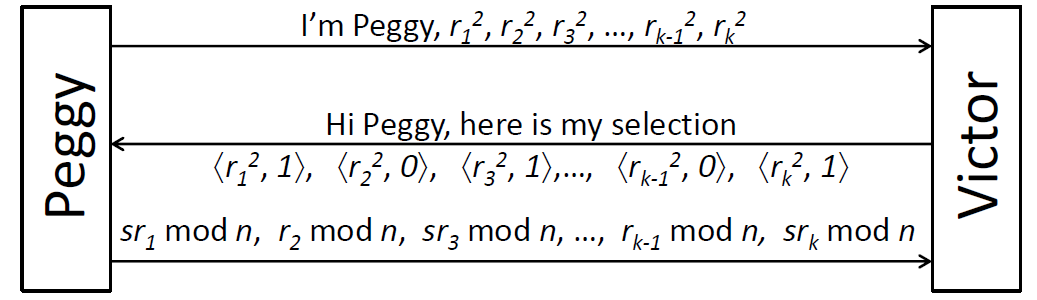
\includegraphics[scale=0.6, keepaspectratio]{Immagini/chiave_pubblica/zkasmsr_auth.png}}
	\caption{}
\end{figure}
Supponiamo che Fred voglia impersonare Peggy. L'etichettatura scelta in modo casuale da Victor implica che Fred ha una probabilità del 50\% di rispondere in modo corretto ad ogni $r_{i}^2$. Fred potrebbe generarsi autonomamente gli $r_{i}$, ma in tal caso non saprebbe rispondere agli $r_{i}^2$ con etichetta 1 oppure potrebbe usare un insieme di $r_{i}^2$ etichettati in passato con 1 in una precedente autenticazione, ma allora non conoscerebbe i corrispondenti $r_{i}$ e non saprebbe rispondere nel caso in cui l'etichetta è 0. Se $k$ è sufficientemente grande la probabilità che Fred impersoni correttamente Peggy tende a 0. \\ \\
In assenza di etichette 0 il protocollo si semplificherebbe: Peggy si limiterebbe ad inviare delle coppie $<r_{i}^2, sr_{i} \, mod \, n>$, tuttavia non si avrebbe più un protocollo a conoscenza zero, poiché Fred potrebbe usare una precedente sequenza inviata di Peggy ed impersonarla con successo. \\ \\
ZKAS basato su MSR è molto più efficiente di RSA. Infatti, assumendo $k = 30$, Peggy deve effettuare 45 operazioni modulari (30 quadrati più una media di 15 moltiplicazioni per $s$) e Victor deve effettuare lo stesso numero di operazioni di Peggy; usando RSA Peggy deve eseguire una esponenziazione modulare che consiste in una media di 768 moltiplicazioni modulari mentre Victor se la cava con 3 moltiplicazioni nel caso in cui $e = 3$.
